\documentclass[12pt,letterpaper]{book}
\usepackage{mathptmx}
\usepackage[latin1]{inputenc}
\usepackage[spanish,es-tabla]{babel}
\usepackage{amsmath}
\usepackage{amssymb, amsfonts, latexsym, cancel}
\usepackage{transparent}
\usepackage{eso-pic,graphicx}
\usepackage{epstopdf}
\usepackage{float}
\usepackage{subfigure}
\usepackage{array}
\usepackage{longtable}
\usepackage[left=2cm,right=2cm,top=2cm,bottom=2cm]{geometry}
\usepackage{bm}
\usepackage{appendix}
\usepackage{subfigure}
\usepackage[subfigure]{tocloft}
\usepackage{multirow} % para las tablas
\usepackage{longtable}
\usepackage{lipsum}
\usepackage[breaklinks=true]{hyperref}
\usepackage[acronym,section=section]{glossaries}
\usepackage{fancyhdr, lastpage}
\usepackage{afterpage}
\usepackage{caption,newfloat}
%\usepackage{natbib}
\usepackage{apacite}
%%%%%%%%%%%%%%%%%%%%%%%%%%%%%%%%%%%%%%%%%%%%%%%%%%
% Agregar una pagina en blanco
\newcommand\blankpage{%
    \null
    \thispagestyle{empty}%
    \addtocounter{page}{-1}%
    \newpage}
%%%%%%%%%%%%%%%%%%%%%%%%%%%%%%%%%%%%%%%%%%%%%%%%%%
% Modificacion de estilos de encabezados y pie de pagina
\fancypagestyle{plain}{
  \fancyhf{}% Clear header/footer
  \fancyfoot[R]{\thepage}% Right footer
  \renewcommand{\headrulewidth}{0.0pt}%
}
\pagestyle{plain}% Set page style to plain.
%%%%%%%%%%%%%%%%%%%%%%%%%%%%%%%%%%%%%%%%%%%%%%%%%%
% Modificar los niveles de nuemeracionº
\setcounter{secnumdepth}{4}
%%%%%%%%%%%%%%%%%%%%%%%%%%%%%%%%%%%%%%%%%%%%%%%%%%
% Modificacion de sangria
\parindent=0cm 
%%%%%%%%%%%%%%%%%%%%%%%%%%%%%%%%%%%%%%%%%%%%%%%%%%
% configuracion de anexos
\renewcommand{\appendixname}{Anexos}
\renewcommand{\appendixtocname}{Anexos}
\renewcommand{\appendixpagename}{Anexos}
%%%%%%%%%%%%%%%%%%%%%%%%%%%%%%%%%%%%%%%%%%%%%%%%%%
% Glosario correspondiente
% \gls{nombre} referenciar la palabra al glosario
% \acrfull{NOMBRE} referenciar el acronimo 
% \acrshort{NOMBRE} Escribir la descripcion del acronimo
% \newglossaryentry{nombre} 
% {
% name={Nombre},
% description={desc}
% }
 \newglossaryentry{MovUni} 
 {
 name={movimiento unilateral},
 description={Movimiento la cual emplea las articulaciones de un lado del cuerpo humano, ejemplo una patada (Debido que se puede patear del lado derecho o izquierdo)}
 }
 \newglossaryentry{visArt} 
 {
 name={visi\'on artificial},
 description={Campo de la  inteligencia artificial que permite adquirir, procesar y comprender las im\'agenes del mundo real}
 }
 \newglossaryentry{telem} 
 {
 name={telemetr\'ia},
 description={Tecnolog\'ia que permite la medici\'on de magnitudes f\'isicas}
 }

 \newglossaryentry{brad} 
 {
 name={base radial},
 description={Procedimiento de redes neuronales que calculan la salida en funci\'on de la distancia de un punto respecto a un punto central }
 }
 
  \newglossaryentry{sigm} 
 {
 name={sigmoide},
 description={Funci\'on matem\'atica, que se utiliza para suavizar los modelos de aprendizaje, cuya forma es de una S }
 }
 
   \newglossaryentry{gaus} 
 {
 name={gaussiana},
 description={En t\'erminos de estad\'isticas, representa la distribuci\'on normal de un grupo de datos}
 }
 
    \newglossaryentry{arbdec} 
 {
 name={\'arbol de decisi\'on},
 description={Modelo de clasificador que se divide por distintos nodos de decisiones, para llegar a una respuesta (hoja)}
 }
 
    \newglossaryentry{knnia} 
 {
 name={K vecinos pr\'oximos},
 description={M\'etodo clasificador supervisado, que sirve para estimar la funci\'on de densidad respecto a un conjunto de datos cercanos al dato que se desea pronosticar}
 } 
 
     \newglossaryentry{redneu} 
 {
 name={red neuronal},
 description={Paradigma de aprendizaje y procesamiento autom\'atico, cuya estructura esta formado por un sistema de interconexi\'on de neuronas que colaboran para producir una o varias salidas}
 }
 
      \newglossaryentry{bayesian} 
 {
 name={clasificador bayesiano},
 description={Clasificador probabil\'istico fundamento en el teorema de bayes (probabilidad dado uno o m\'as eventos)}
 }
      \newglossaryentry{matcov} 
 {
 name={matriz de covarianza},
 description={Matriz cuadrada que contiene las varianzas y covarianzas asociadas a diferentes variables}
 } 
      \newglossaryentry{elmia} 
 {
 name={m\'aquina de aprendizaje extremo},
 description={M\'aquina que se conforma de redes neuronales, cuya esencia es que la capa oculta de la red se construye con un entrenamiento r\'apido y con poca participaci\'on humana}
 }  
       \newglossaryentry{svmia} 
 {
 name={m\'aquina de soporte vectorial},
 description={M\'etodo clasificador, la cual separa un conjunto de datos mediante un hiperplano de separaci\'on}
 }
 
  \newglossaryentry{Heur} 
 {
 name={heur\'istica},
 description={M\'etodo basado en la experiencia (informaci\'on previa), que puede utilizarse para resolver problemas }
 }

  \newglossaryentry{diseuc} 
 {	
 name={distancia euclidiana},
 description={Distancia entre dos puntos}
 }
 
 
 \newglossaryentry{pixeles} 
 {
 name={p\'ixeles},
 description={Unidades b\'asicas de una imagen que obtiene el valor de un color}
 }
 
 \newglossaryentry{infrarrojo} 
 {
 name={infrarrojo},
 description={Radiaci\'on electromagn\'etica que emite un cuerpo, independiente a que exista otro tipo de luz}
 }
 
  \newglossaryentry{TOF} 
 {
 name={tiempo de vuelo},
 description={T\'ecnica que se emplea para calcular distancia entre objetos}
 }
% \newacronym{NAME}{NAME}{DESCRIPCION}
\newacronym{TRESD}{3D}{tercera dimensi\'on}
\newacronym{RGBD}{RGB-D cameras}{c\'amaras con sensor de profundidad}
\newacronym{FPS}{FPS}{fotogramas por segundo}
\newacronym{FOV}{FOV}{campo de visi\'on}
\newacronym{NUI}{NUI}{interfaz de usuario natural}
\newacronym{SDK}{SDK}{Kit de desarrollo de software}
\newacronym{API}{API}{Interfaz de programación de aplicaciones}
\newacronym{LED}{LED}{Diodo de emisor de luz}
\newacronym{RAM}{RAM}{Memoria de acceso aleatorio}
\newacronym{XEF}{XEF}{extended event files}
\newacronym{RFR}{RFR}{Random Forest Regression}
\newacronym{AdaBoost}{AdaBoost}{Adaptive Boosting}
\newacronym{VGB}{VGB}{Visual Gesture Builder}
\newacronym{xIIT}{xIIT}{Entrenamientos por intervalos de alta, media o baja intensidad}
\newacronym{ATP}{ATP}{Trifosfato de adenosina}
\newacronym{CP}{CP}{Fosfato de creatina}
\newacronym{ADP}{ADP}{Difosfato de adenosina}

\makeglossaries
%%%%%%%%%%%%%%%%%%%%%%%%%%%%%%%%%%%%%%%%%%%%%%%%%%
% Definicion de ecuaaciones
\DeclareFloatingEnvironment[
  fileext=lofor,
  listname=Formula, % English name
  name=List of Formulas, % English name
  placement=tbp,
]{formula}

\addto\captionsspanish{% provide translations for Portuguese
  \renewcommand{\formulaname}{Ecuaci\'on}%
  \renewcommand{\listformulaname}{\'Indice de Ecuaciones}%
}

%%%%%%%%%%%%%%%%%%%%%%%%%%%%%%%%%%%%%%%%%%%%%%%%%%
% Definicion de ecuaaciones
\DeclareFloatingEnvironment[
  fileext=loc,
  listname=Chart, % English name
  name=List of Charts, % English name
  placement=tbp,
]{chart}

\addto\captionsspanish{% provide translations for Portuguese
  \renewcommand{\chartname}{Gr\'afico}%
  \renewcommand{\listchartname}{\'Indice de Gr\'aficos}%
}
%%%%%%%%%%%%%%%%%%%%%%%%%%%%%%%%%%%%%%%%%%%%%%%%%%
% Estilos de bibliografia
%\bibliographystyle{apalike} 
\bibliographystyle{apacite}
%%%%%%%%%%%%%%%%%%%%%%%%%%%%%%%%%%%%%%%%%%%%%%%%%%
\begin{document}
\frontmatter
\begin{titlepage}
\begin{center}
\AddToShipoutPictureBG*{\transparent{0.25}
\includegraphics[width=\paperwidth,height=\paperheight]{graphics/logo.jpg}}
{\LARGE \textbf{UNIVERSIDAD RAFAEL LAND\'IVAR}}\\[0.1cm]
{\normalsize FACULTAD DE INGENIER\'IA}\\[0.1cm]
{\normalsize DEPARTAMENTO DE INGENIER\'IA EN INFORM\'ATICA Y SISTEMAS}\\[4cm]
{\huge \textbf{Aplicaci\'on del algoritmo de Random Forest Regression para la detecci\'on de los pasos requeridos de un movimiento v\'alido mediante la utilizaci\'on del dispositivo Kinect V2}}\\[0.1cm]
{\LARGE PROYECTO DE INGENIER\'IA}
\vfill
DIEGO JOS\'E ORELLANA BOJORQUEZ\\[0.1cm]
CARN\'E 10101-14\\[2cm]
Guatemala, Enero de 2020\\[0.1cm]
Campus Central
\afterpage{\blankpage}
\end{center}
\end{titlepage}
\begin{center}
\AddToShipoutPictureBG*{\transparent{0.25}
\includegraphics[width=\paperwidth,height=\paperheight]{graphics/logo.jpg}}
{\LARGE \textbf{UNIVERSIDAD RAFAEL LAND\'IVAR}}\\[0.1cm]
{\normalsize FACULTAD DE INGENIER\'IA}\\[0.1cm]
{\normalsize DEPARTAMENTO DE INGENIER\'IA EN INFORM\'ATICA Y SISTEMAS}\\[4cm]
{\huge \textbf{Aplicaci\'on del algoritmo de Random Forest Regression para la detecci\'on de los pasos requeridos de un movimiento v\'alido mediante la utilizaci\'on del dispositivo Kinect V2.}}\\[0.1cm]
{\LARGE PROYECTO DE INGENIER\'IA}
\vfill
{\LARGE Presentada ante el Consejo de la Facultad de Ingenier\'ia}
\vfill
{\LARGE Por:}\\[0.1cm]
{\LARGE \textbf{DIEGO JOS\'E ORELLANA BOJORQUEZ}}
\vfill
Previo a optar el t\'itulo de:\\[0.1cm]
Ingeniero en Inform\'atica y Sistemas
\vfill
En el grado acad\'emico de:\\[0.1cm]
Licenciado
\vfill
Guatemala, Enero de 2020\\[0.1cm]
Campus Central
\end{center}
%%%%%%%%%%%%%%%%%%%%%%%%%%%%%%%%%%%%%%%%%%%%%%%%%
% notificaci�n
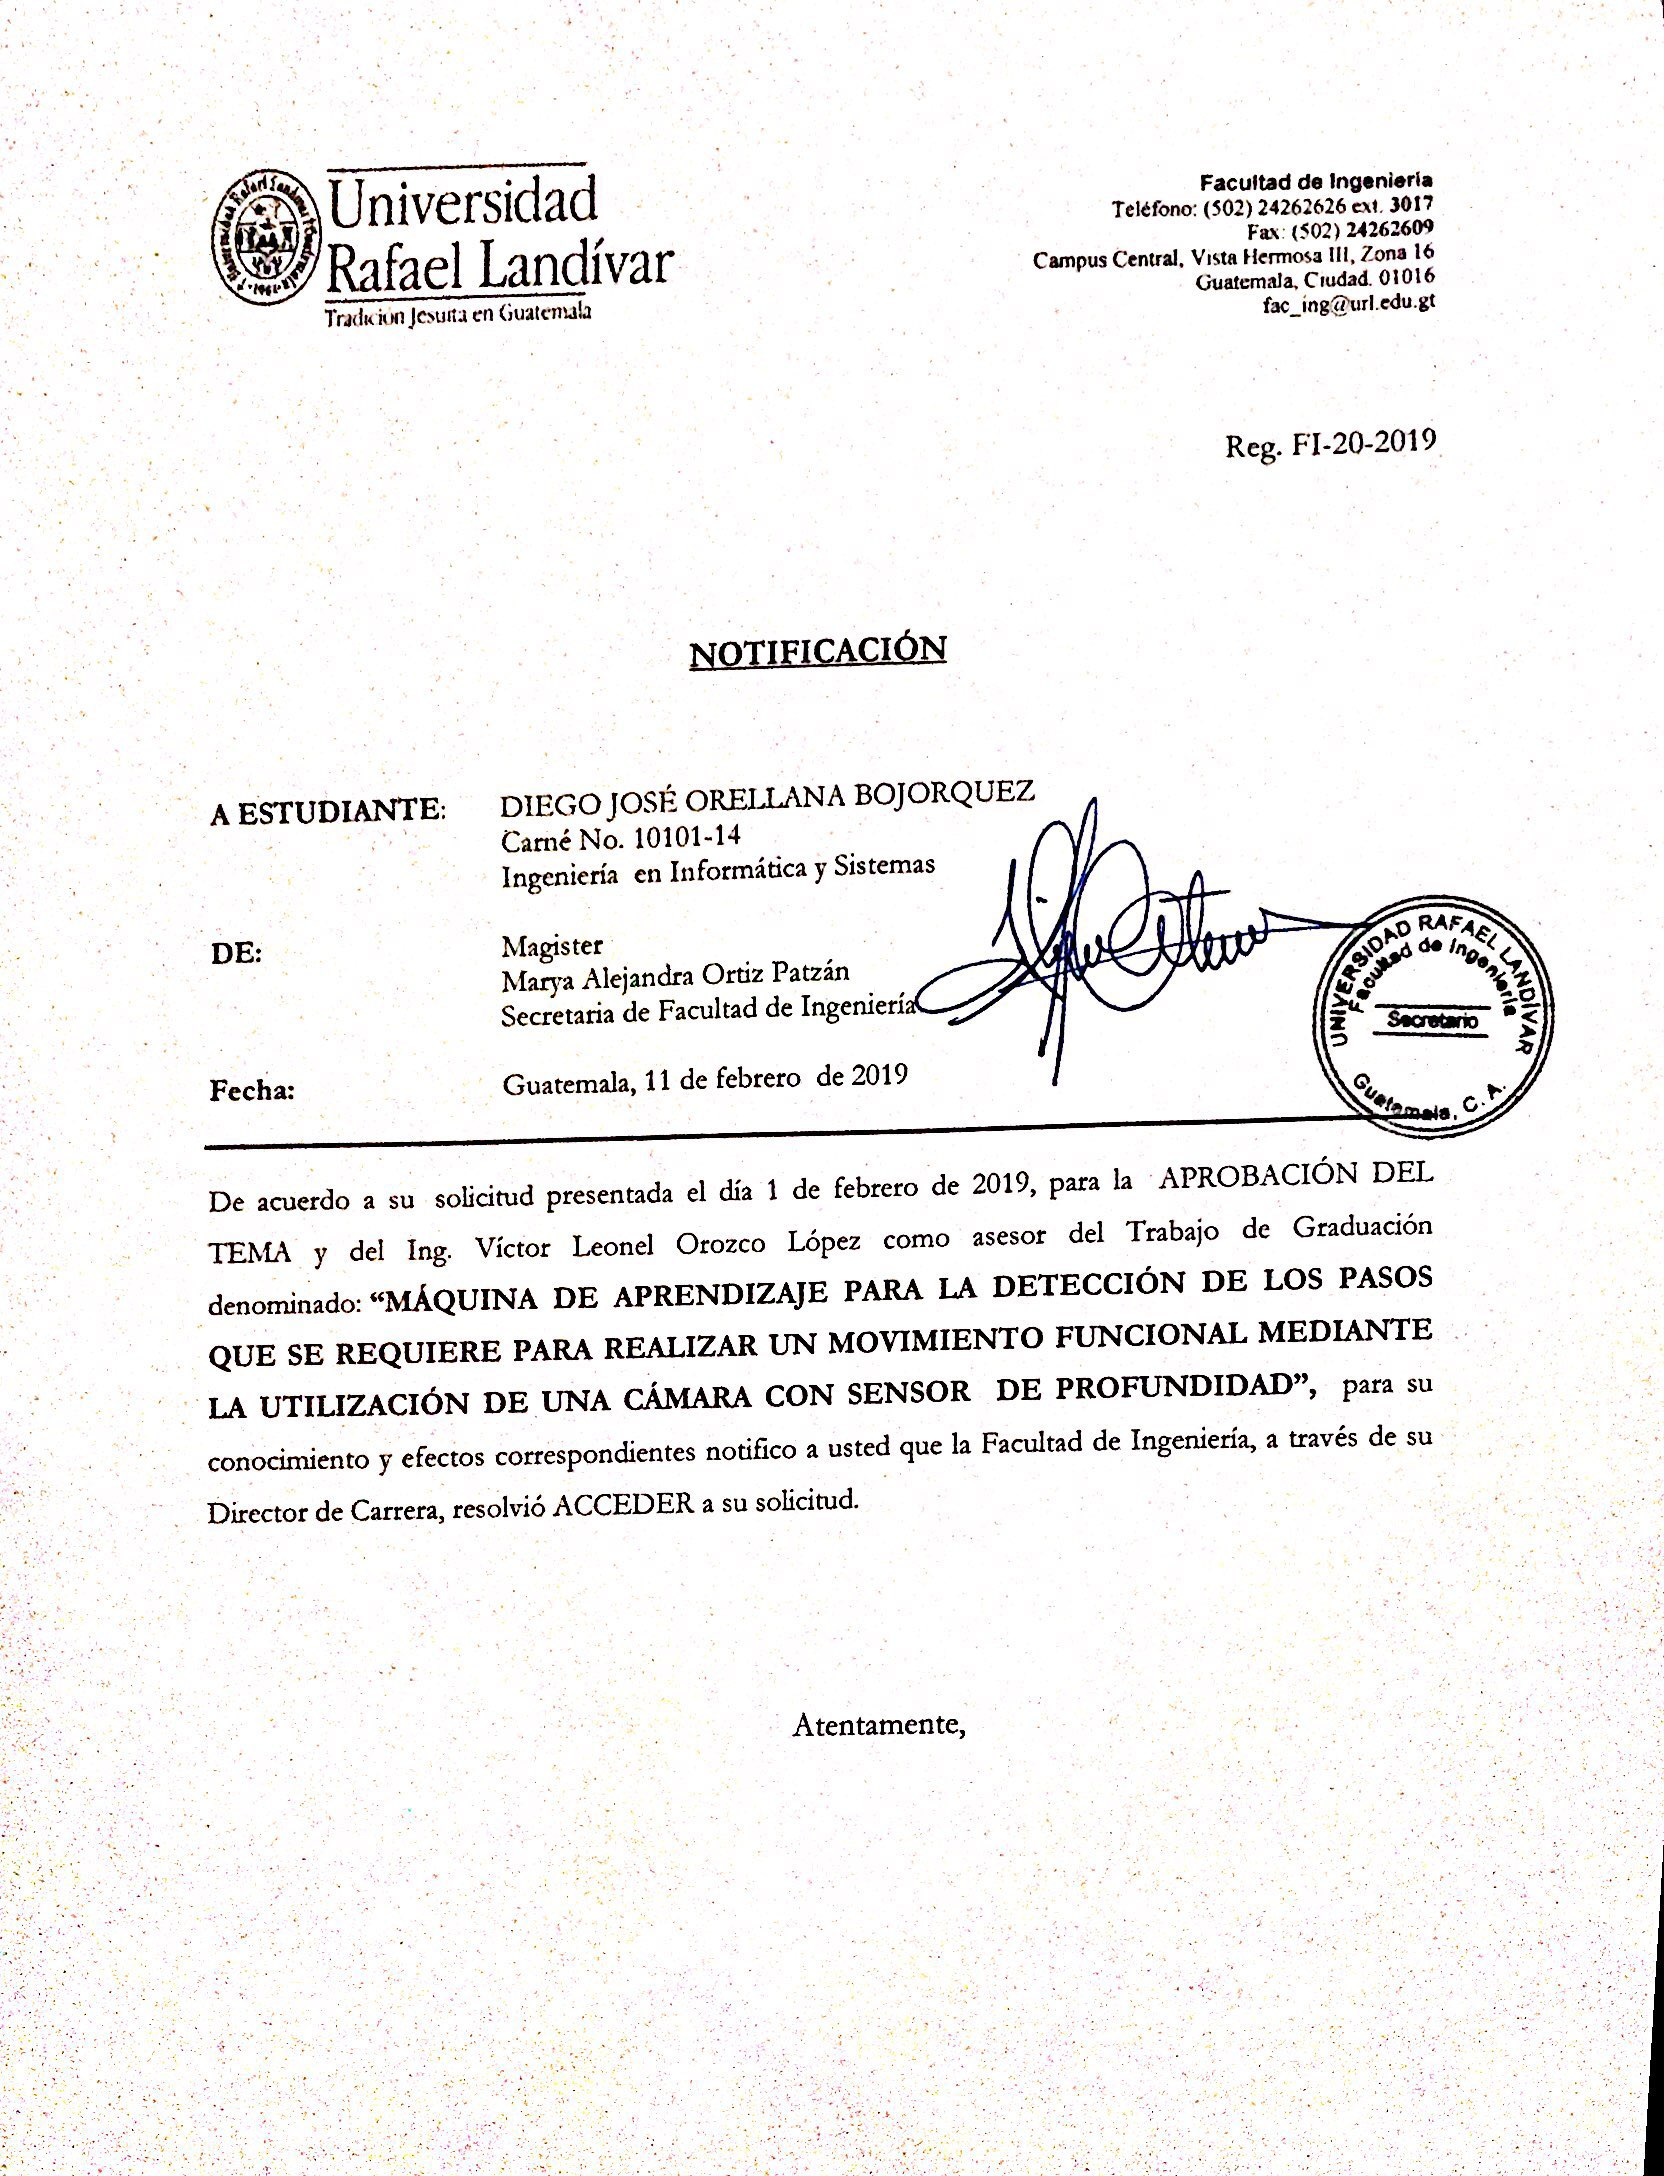
\includegraphics[width=18cm,height=22cm]{graphics/notificacion-tesis.jpg}
%%%%%%%%%%%%%%%%%%%%%%%%%%%%%%%%%%%%%%%%%%%%%%%%%
\afterpage{\blankpage}
\newpage
{\LARGE \textbf{Agradecimientos}}\\[2cm]
\begin{itemize}
\item A Dios, por ser alguien que me escucha en todo momento.
\item A mi mam\'a, gracias a ella he llegado tan lejos, adem\'as de estar siempre conmigo en las buenas y en las malas. 
\item A mi hermanos, por tenerme paciencia y confiar en m\'i en todo momento.
\item A mi pap\'a, por acompa\~narme siempre.
\item A mis amigos de la universidad, por ser una gran promoci\'on unida y apoyarnos en todo momento.
\item A mis amigos del colegio, por mantener nuestra amistad y vernos crecer.
\item Ingenieros Stanly Bola\~nos y Victor Orozco, por apoyarme en todo el proceso de trabajo de investigaci\'on.
\item Departamento de deportes de la universidad Rafael Land\'ivar, por confiar en mi proyecto de ingenier\'ia.
\end{itemize}
\begin{center}
Diego Orellana.
\end{center}
\afterpage{\blankpage}
\newpage
\tableofcontents.
\listoffigures.
\listoftables.
\listofcharts.
\listofformulas.
\listofcodes.
\mainmatter
%index
\chapter{INTRODUCCI�N}
\section{LO ESCRITO SOBRE EL TEMA}
\section{MARCO TE�RICO}
\chapter{PLANTEAMIENTO DEL PROBLEMA}
\section{OBJETIVOS}
\subsection{OBJETIVO GENERAL}
\subsection{OBJETIVOS ESPEC�FICOS}
\section{HIP�TESIS}
\section{VARIABLES}
\subsection{VARIABLES DEPENDIENTES}
\subsection{VARIABLES INDEPENDIENTES}
\section{DEFINICI�N DE LAS VARIABLES}
\subsection{DEFINICI�N CONCEPTUAL}
\subsection{DEFINICI�N OPERACIONAL}
\section{ALCANCES}
\section{L�MITES}
\section{APORTE}
\chapter{M�TODO}
\section{SUJETOS}
\subsection{PRIMER TIPO}
\subsection{SEGUNDO TIPO}
\section{UNIDADES DE AN�LISIS}
\section{INSTRUMENTOS}
\section{PROCEDIMIENTO}
\section{DISE�O Y METODOLOG�A ESTAD�STICA}
\subsection{DISE�O EXPERIMENTAL}
\subsubsection{EXPERIMENTOS}
\subsubsection{TRATAMIENTOS Y REPETICIONES EN LOS EXPERIMENTOS}
\chapter{PRESENTACI�N Y AN�LISIS DE RESULTADOS}
\chapter{DISCUSI�N}
\chapter{CONCLUSIONES}
\chapter{RECOMENDACIONES}
\backmatter
\bibliography{backmatter/bibliografia}
\appendix
\clearpage
\addappheadtotoc
\appendixpage

\end{document}